% This LaTeX was auto-generated from MATLAB code.
% To make changes, update the MATLAB code and export to LaTeX again.

\documentclass{article}

\usepackage[utf8]{inputenc}
\usepackage[T1]{fontenc}
\usepackage{lmodern}
\usepackage{graphicx}
\usepackage{color}
\usepackage{hyperref}
\usepackage{amsmath}
\usepackage{amsfonts}
\usepackage{epstopdf}
\usepackage[table]{xcolor}
\usepackage{matlab}

\sloppy
\epstopdfsetup{outdir=./}
\graphicspath{ {./angular_rates1_live_images/} }

\begin{document}

\begin{matlabcode}
clc; clear

% Load Data
data = load('2023_10_13_002_RWHEEL_05_02');
time = data(:,1); %[s]
gyro_output = data(:,2); %[rad/s]
input = data(:,3); %[rpm]

% Adjust Time Vector
time = time - 13523.26;
time(1) = 0;

% Convert rpm -> rad/s
input = input./60; %[rps]
input = input * 2*pi;

% Plot vs Time
figure();
plot(time,input)
hold on
plot(time,gyro_output)
hold off
grid on;grid minor
xlabel('Time [s]')
ylabel('Angular Rate [rad/s]')
legend('Input Rate','Gyro Output Rate')
title('Angular Rates vs Time')
\end{matlabcode}
\begin{center}
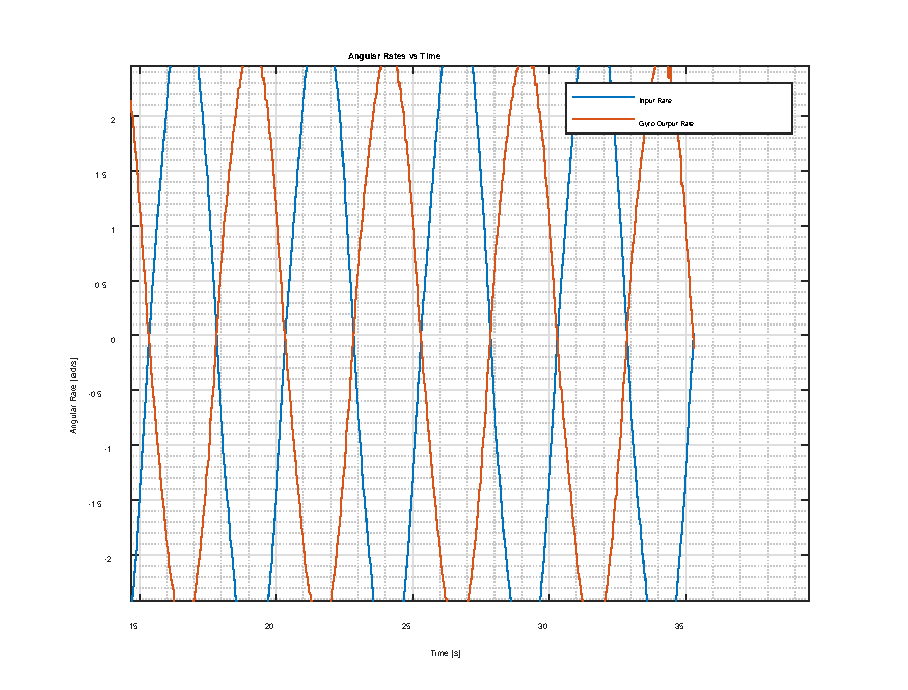
\includegraphics[width=\maxwidth{56.196688409433015em}]{figure_0.eps}
\end{center}
\begin{matlabcode}

% Plot Input vs Output
figure();
scatter(input,gyro_output,'.')
hold on
xlabel('Input Rate [rad/s]')
ylabel('Output Rate [rad/s]')
title('Gyro Data')
grid on; grid minor

% Determine K
p = polyfit(input,gyro_output,1);
K = p(1).*input + p(2);

% Plot K
plot(input,K,'LineWidth',2)

% Detrmine b
b = mean(gyro_output);
b = b + zeros(length(input),1);

% Plot b
plot(input,b,'--k')
legend('Data','Adjusted Scale Factor (K)','Bias (b)')
hold off
\end{matlabcode}
\begin{center}
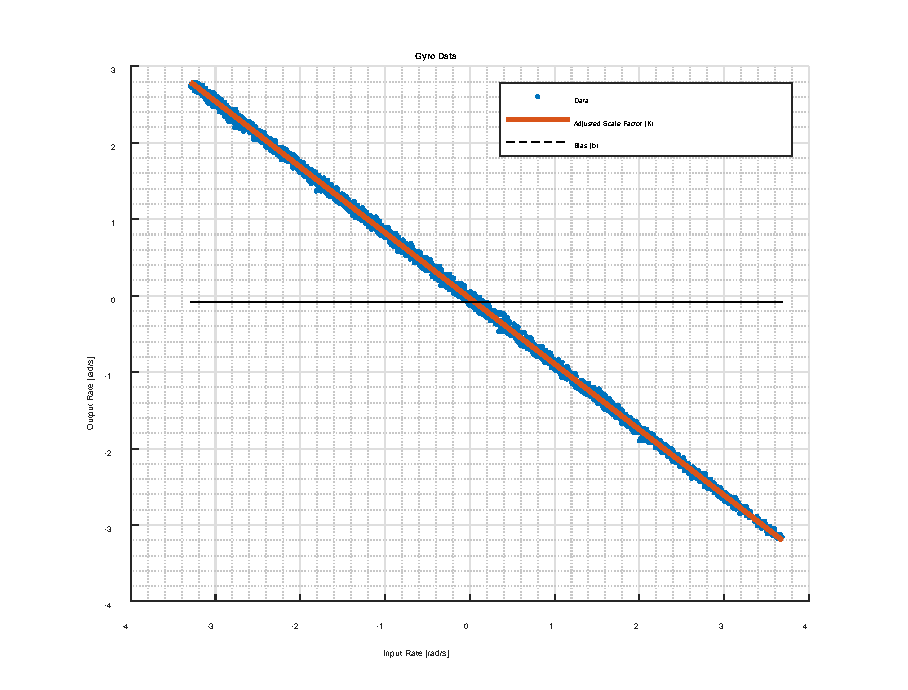
\includegraphics[width=\maxwidth{56.196688409433015em}]{figure_1.eps}
\end{center}
\begin{matlabcode}

% Adjust Gyro Measurements
adj_gyro = p(1)*gyro_output + b;

% Plot New vs Time
figure();
plot(time,input)
hold on
plot(time,adj_gyro)
legend('Input Rate','Calibrated Output Rate')
hold off
grid on; grid minor
xlabel('Time [s]')
ylabel('Angular Rate [rad/s]')
title('Angular Rates (adjusted) vs Time')
\end{matlabcode}
\begin{center}
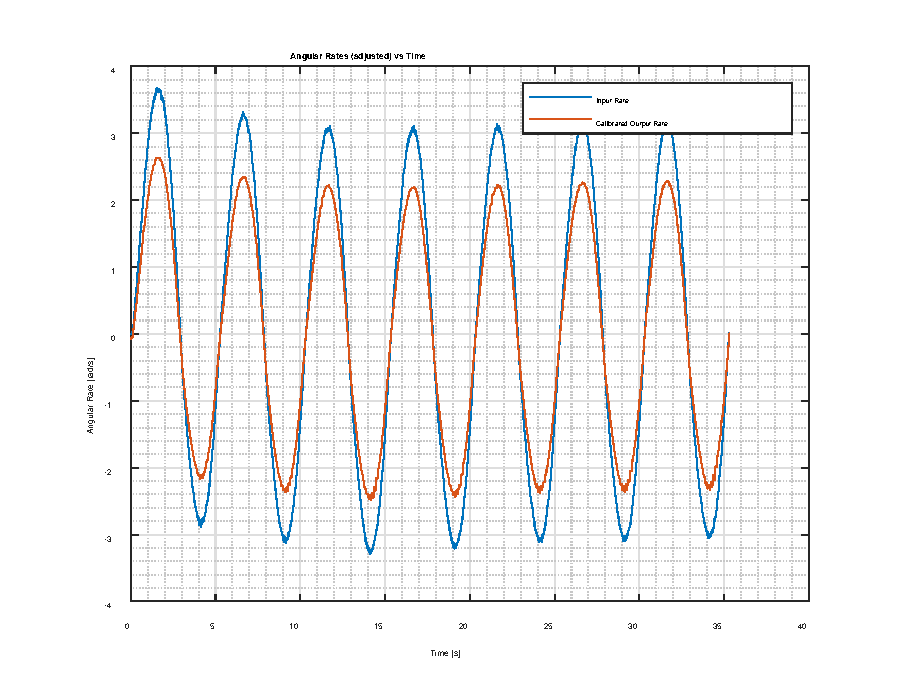
\includegraphics[width=\maxwidth{56.196688409433015em}]{figure_2.eps}
\end{center}
\begin{matlabcode}

% Find and Plot Differences - Rate
difference_rate = input - adj_gyro;

figure();
plot(time,difference_rate)
title('Angular Rate Measurement Error')
xlabel('Time [s]')
ylabel('Difference in Angular Rate [rad/s]')
grid on; grid minor;
\end{matlabcode}
\begin{center}
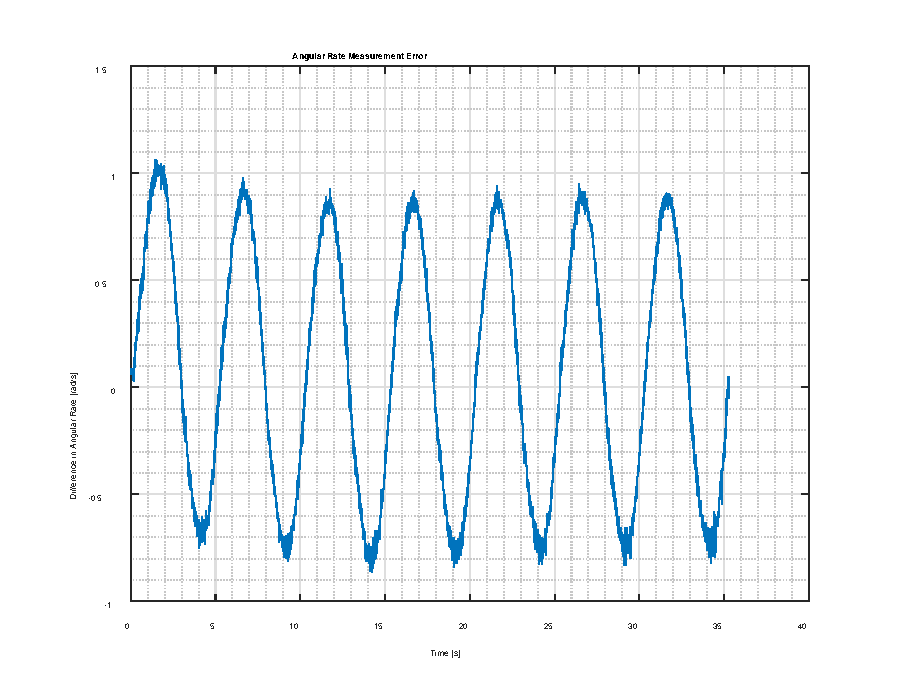
\includegraphics[width=\maxwidth{56.196688409433015em}]{figure_3.eps}
\end{center}
\begin{matlabcode}

% Find and Plot Angular Position
input_pos = input .* time;
adj_gyro_pos = adj_gyro .* time;

figure();
plot(time,input_pos)
hold on
plot(time,adj_gyro_pos)
hold off
grid on; grid minor
title('Angular Position vs Time')
ylabel('Angular Position [rad]')
xlabel('Time [s]')
legend('Input Position','Calibrated Output Position')
\end{matlabcode}
\begin{center}
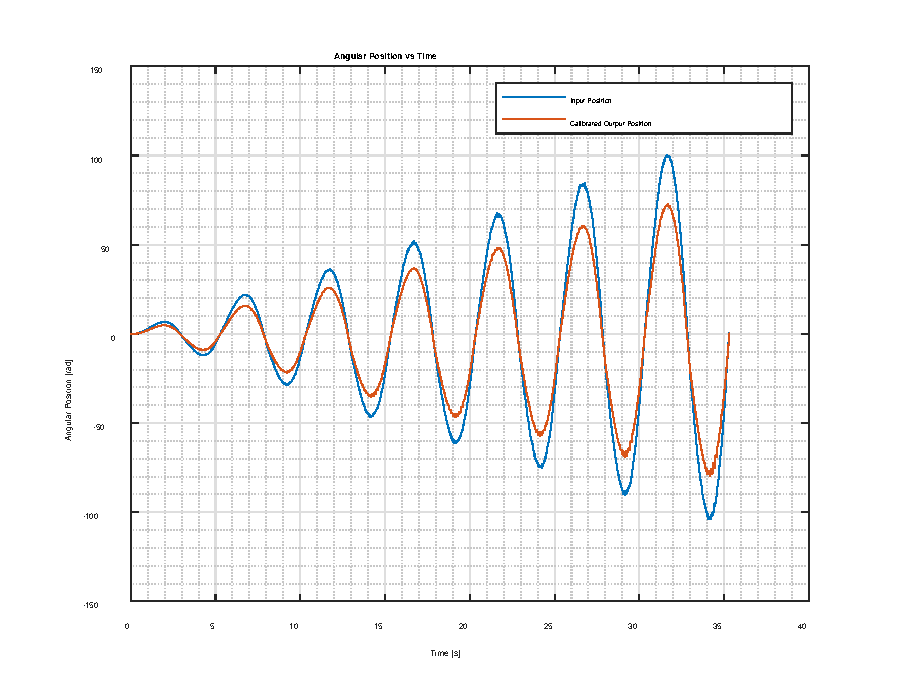
\includegraphics[width=\maxwidth{56.196688409433015em}]{figure_4.eps}
\end{center}
\begin{matlabcode}

% Find and Plot Differences - Position
difference_pos = input_pos - adj_gyro_pos;

figure();
plot(time,difference_pos)
title('Angular Position Measurement Error')
xlabel('Time [s]')
ylabel('Difference in Angular Position [rad]')
grid on; grid minor
\end{matlabcode}
\begin{center}
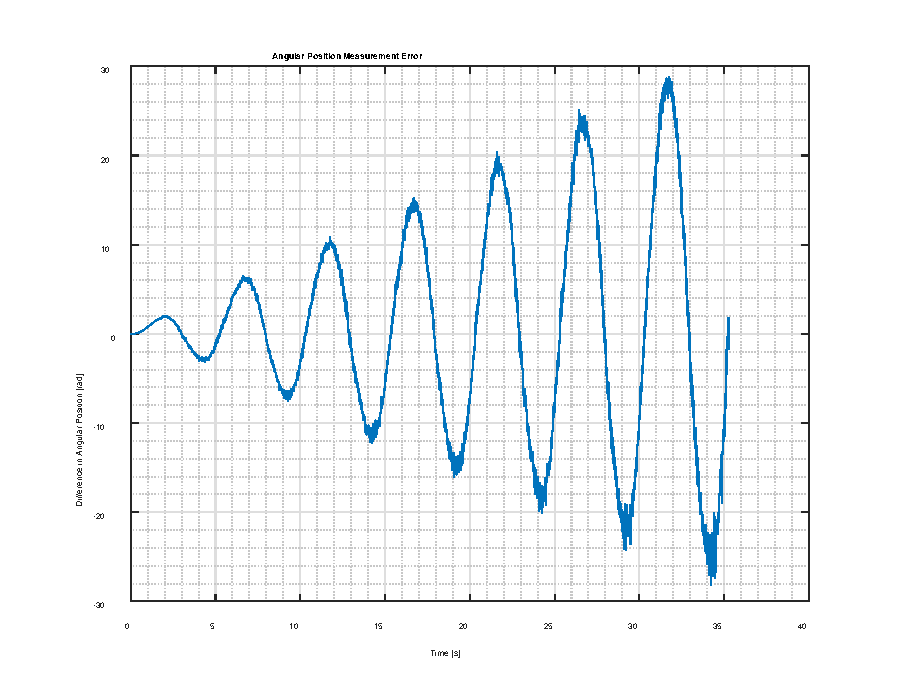
\includegraphics[width=\maxwidth{56.196688409433015em}]{figure_5.eps}
\end{center}
\begin{matlabcode}

% Angular Position as a Funciton of Input Rate
figure();
plot(input,difference_pos)
grid on; grid minor
title('Angular Position as a Funciton of Input Rate')
xlabel('Input Rate [rad/s]')
ylabel('Angular Position Error [rad]')
\end{matlabcode}
\begin{center}
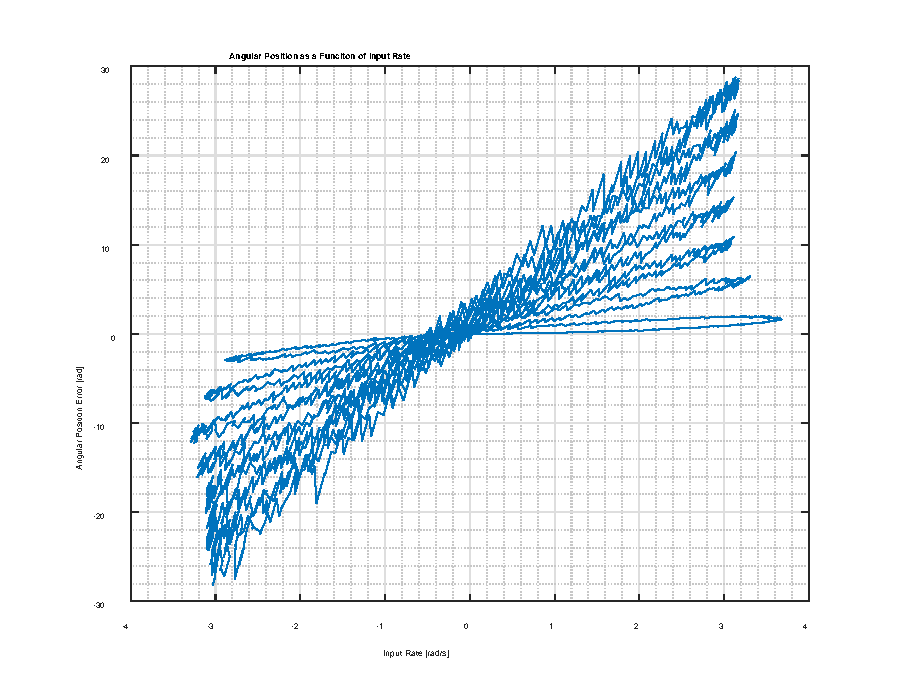
\includegraphics[width=\maxwidth{56.196688409433015em}]{figure_6.eps}
\end{center}
\begin{matlabcode}

\end{matlabcode}

\end{document}
